% !TeX root = ../libro.tex
% !TeX encoding = utf8

\setchapterpreamble[c][0.75\linewidth]{%
	\sffamily
	% Introducción al capitulo
	\par\bigskip
}
\chapter{Teoría de Grafos}\label{ch:segundo-capitulo}
Las definiciones y conceptos de este capítulo han sido extraídos de la referencia \cite{algorithms}.

\section{Conceptos básicos y propiedades asociadas a grafos}
Vamos a comenzar viendo algunas definiciones y conceptos básicos.

\begin{definicion}
	Un \textit{grafo no  dirigido} es un par (\textbf{V}, \textbf{E}), donde \textbf{V} es un conjunto no vacío, a cuyos elementos denominaremos \textit{vértices} o \textit{nodos}, y \textbf{E} es un conjunto finito de pares de elementos de \textbf{V}, a los que llamaremos \textit{aristas} o \textit{lados}.
\end{definicion}

\begin{itemize}
	\item A los nodos $v_1$ y $v_2$ que forman una arista $e=\{v_1, v_2\}$ se les llama \textit{extremos} de $e$. Cuando esto ocurra, se dirá que los vértices $v_1$ y $v_2$ son \textit{adyacentes} o \textit{vecinos}.
	
	\item Se dirá que una arista $e$ es \textit{incidente} con un vértice $v$ cuando $v$ sea uno de sus extremos. En dicho caso se dirá que $e$ \textit{incide} en $v$.
\end{itemize}

\begin{definicion}
	Se denominará \textit{grado de incidencia} de un vértice $v\in V$ (que denotaremos por $g(v)$), al número de aristas incidentes con $v$.
\end{definicion}

Por conveniencia, no consideraremos lados que conecten un vértice consigo mismo, es decir, lados del tipo $\{v, v\}$. \\

En este tipo de grafos no se tiene en cuenta el orden en el que aparecen los vértices en una arista, es decir,  $e=\{v_1, v_2\}=\{v_2, v_1\}$. El siguiente tipo de grafo sí que diferencia entre ambas aristas, incluyendo una orientación sobre las mismas.

\begin{definicion}
	Un \textit{grafo dirigido} es un grafo $G$ cuyas aristas cuentan con una orientación, en este caso pasarán a ser llamadas \textit{arcos}. En este caso denotaremos los arcos como $e=(v_1,v_2)$, siendo $e$ un arco orientado de $v_1$ hacia $v_2$.
\end{definicion}

Cuando planteamos un grafo asociado a un problema, las aristas suelen ser caminos entre nodos, con un coste asociado, para introducir estos costes definimos el siguiente tipo de grafo.

\begin{definicion}
	Un \textit{grafo ponderado} (o grafo con pesos), es una terna $(V,E,\omega)$ donde el par $(V,E)$ representa un grafo (dirigido o no dirigido), y $\omega:E\rightarrow\mathbb{R}$ es una aplicación que asigna a cada arista o arco el peso asociado.
\end{definicion}

En la \autoref{fig:graf-ej} podemos observar ejemplos de las definiciones anteriores, por ejemplo, los vértices $0$ y $2$ son adyacentes, y el grado de incidencia del vértice $a$ es $4$. \\

\begin{figure}[htb]
	\centering
	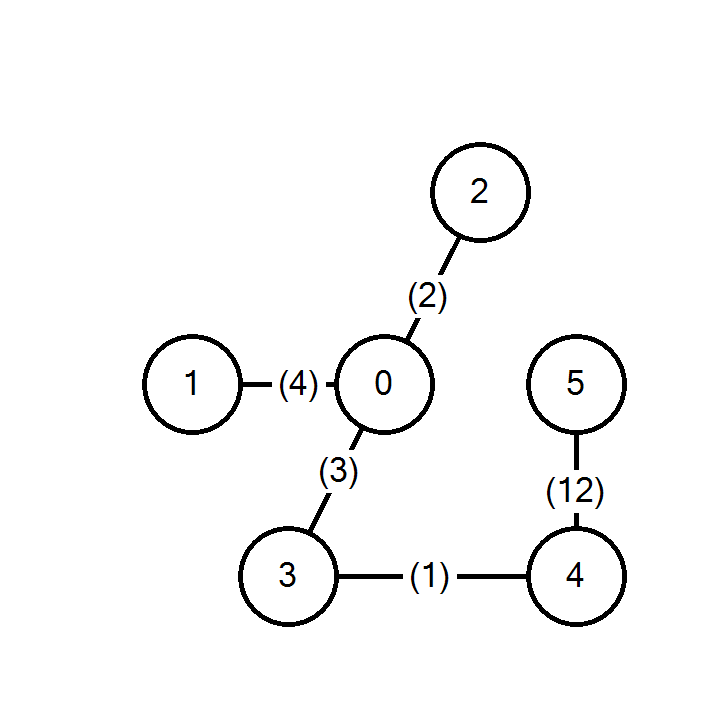
\includegraphics[width=0.4\linewidth]{graf-ej-1}
	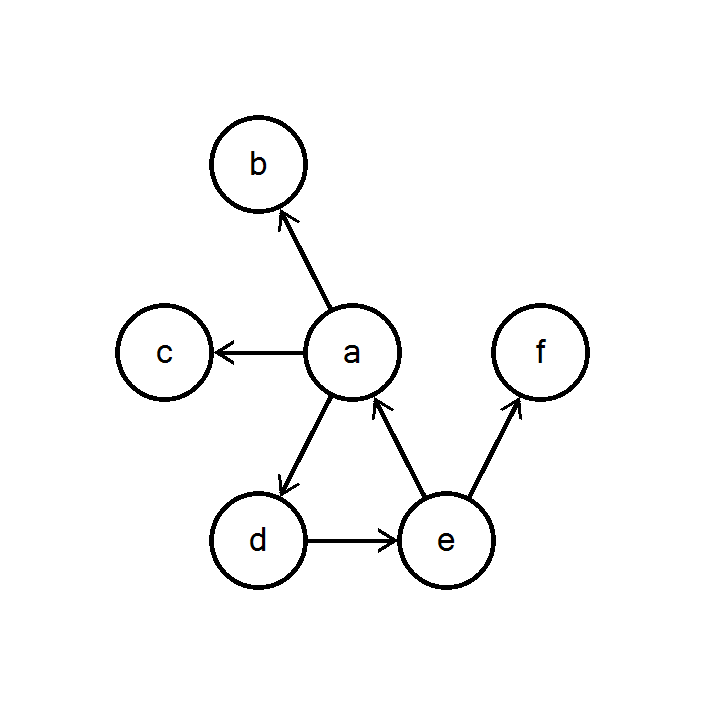
\includegraphics[width=0.4\linewidth]{graf-ej-2}
	\caption{Ejemplo de grafo no dirigido ponderado, izquierda, y grafo dirigido no ponderado, derecha.}
	\label{fig:graf-ej}
\end{figure}

A continuación plantearemos algunas definiciones sobre distintos tipos de grafos.

\begin{definicion}
	Un \textit{grafo finito} es un grafo $G$ (dirigido o no dirigido), con un número finito de vértices, es decir, el conjunto $V$ es finito.
\end{definicion}

\begin{definicion}
	Un \textit{grafo de incidencia finita} es un grafo $G$ donde el grado de incidencia de cada vértice es finito, es decir, $g(v)$ es finito para cada $v\in V$.
\end{definicion}

\begin{definicion}
	Dado un grafo $G=(V,E)$: 
	\begin{itemize}
		\item Se dirá que $G'=(V',E')$ es un \textit{subgrafo} de $G$ si $V'\subseteq V$ y $E'\subseteq E$.
		\item Se dirá que $G'=(V,E')$ es un \textit{subgrafo parcial} de $G$ si $E'\subseteq E$.
	\end{itemize} 
\end{definicion}

\begin{definicion}
	Dado un grafo $G=(V,E)$ y $B\subseteq V$, se dirá \textit{subgrafo de G inducido por B} a $G_B=(B,E_B)$ con
	$$E_B=\{(i,j)\in E:\ i,j\in B\}\ |\ E_B=\{\{i,j\}\in E:\ i,j\in B\}$$
\end{definicion}

Un concepto natural que surge al hablar de grafos es el de camino entre dos nodos, definimos a continuación formalmente el concepto tanto del camino como tal como de la longitud del mismo.

\begin{definicion}
	Dado un grafo $G$, un \textit{camino} es una sucesión de vértices $v_1v_2...v_{n+1}$ y aristas $e_1e_2...e_n$ tal que $e_i=\{v_i,v_{i+1}\}$ si es un grafo no dirigido, o bien $e_i=(v_i,v_{i+1})$ si es un grafo dirigido, $\forall i \in \{1,...,n\}$. Para referirnos a un camino de ahora en adelante, utilizaremos la sucesión de vértices $v_1...v_{n+1}$ si no es necesario conocer las aristas en concreto, o $e_1...e_n$ si necesitamos conocerlas.
\end{definicion}

\begin{definicion}
	Un camino se dirá \textit{simple} si ninguno de sus vértices está repetido en el propio camino, es decir, si pasa por sus vértices una única vez.
\end{definicion}

\begin{definicion}
	Dado un grafo $G$, se define un \textit{ciclo}, sobre el mismo, como un camino en el que el nodo inicial y final son el mismo. Diremos también en un grafo ponderado, que un ciclo es \textit{negativo}, si la longitud del mismo es negativa.
\end{definicion}

\begin{definicion}
	Se define la \textit{longitud} de un camino $v_1v_2...v_{n+1}$ con aristas $e_1e_2...e_n$ como sigue: 
	$$Long(v_1v_2...v_{n+1}) = \sum_{i=1}^{n}\omega(e_i)$$
	En caso de que no sea un grafo ponderado, supondremos coste $1$ para todas las aristas, en cuyo caso, la longitud del camino será $n$.
\end{definicion}

Definimos a continuación una función que nos será útil más adelante.

\begin{definicion}\label{def:dist}
	Dado un grafo finito $G=(V,E)$ y $v_0,v_1\in V$ no ponderado o ponderado con pesos estrictamente positivos, Definimos $d:V\times V \rightarrow \mathbb{R}\cup \{\infty\}$ como sigue:
	$$d(v_0,v_1)= \left\{ \begin{array}{lcc}
		min\{Long(v_0...v_1) : v_0...v_1\ camino\ desde\ v_0\ a\ v_1\} &   si\ existe\ camino\ entre\ v_0\ y\ v_1 \\
		\\ \infty &  en\ otro\ caso
	\end{array}
	\right.$$
\end{definicion}

Sabemos que existe el mínimo, pues si no hay ciclos, como los conjuntos de vértices y aristas son finitos, el conjunto de caminos entre dos vértices es también finito. Y, de existir algún ciclo, como no puede ser negativo, repetir el mismo ciclo dentro de un camino aumenta la longitud total, por lo que dichos caminos no pueden ser el mínimo, si nos restringimos a los caminos que no pasan por el ciclo, esta cantidad es finita, al igual que antes. \\

Probaremos a continuación que, tal y como sugiere la definición, $d$ es un distancia.

\begin{proposicion}\label{prop:distancia}
	Sea $G$ un grafo finito no dirigido, no ponderado o ponderado, se verifica que $d:V\times V \rightarrow \mathbb{R}\cup \{\infty\}$ con la definición anterior es una distancia en $G$.
\end{proposicion}

\begin{proof}
	Dado que los únicos caminos de longitud $0$ son aquellos en los que no hay aristas, es claro que $d(v_0, v_1) = 0 \Leftrightarrow v_0 = v_1$. La simetría es clara, pues, en un grafo no dirigido, un camino desde $v_0$ a $v_1$ es también un camino desde $v_1$ a $v_0$, dado que podemos recorrer las aristas en los dos sentidos. Para probar la desigualdad triangular, es decir, $\forall v_0, v_1, v_2 \in V,\ d(v_0,v_1) \leq d(v_0,v_2) + d(v_2,v_1)$, hay que distinguir dos casos, el primero, si no existe ningún camino que conecte $v_0$ con $v_2$ o ningún camino que conecte $v_2$ con $v_1$, en cuyo caso se tendría $d(v_0,v_1)\leq \infty$, por lo que siempre se verifica la desigualdad. En caso contrario, si existieran caminos que conectan $v_0$ con $v_2$ y $v_2$ con $v_1$, respectivamente, sean $c_1$ y $c_2$ caminos con longitud mínima entre $v_0$ y $v_2$, y $v_2$ y $v_1$, el camino $c$ que resulta de unir $c_1$ con $c_2$ es un camino entre $v_0$ y $v_1$ luego, por definición de $d$, se tiene
	$$d(v_0, v_1) \leq Long(c) = Long(c_1)+Long(c_2)=d(v_0,v_2)+d(v_2,v_1)$$
\end{proof}

\begin{proposicion}
	Sea $G$ un grafo dirigido, no ponderado o ponderado con pesos exclusivamente positivos, se verifica que $d:V\times V \rightarrow \mathbb{R}\cup \{\infty\}$ con la definición anterior es una distancia asimétrica en $G$.
\end{proposicion}

Esta proposición no necesita demostración, pues los argumentos utilizados para probar la no negatividad y la desigualdad triangular en la \autoref{prop:distancia} son válidos también para grafos dirigidos.

\begin{definicion}
	Dado un grafo $G=(V,E)$ y un camino $v_0...v_1$ entre los vértices $v_0$ y $v_1$, a dicho camino se le llama \textit{camino de longitud mínima} desde $v_0$ a $v_1$ si y solo si es la geodésica entre $v_0$ y $v_1$, es decir:
	$$Long(v_0...v_1) = d(v_0, v_1)$$
\end{definicion}

\begin{definicion}
	Se define el \textit{grafo de caminos de longitud mínima} con raíz $s$ como un grafo $G$ en el que todo camino entre $s$ y cualquier otro nodo $v$ es de longitud mínima, además, existe al menos un camino entre $s$ y cada nodo de $G$
\end{definicion}

Veremos a continuación un par de propiedades muy interesantes asociadas a los caminos de longitud mínima.

\begin{proposicion}\label{prop:separa_cam_min_long}
	Dado un camino de longitud mínima $v_0...v_i...v_1$ desde $v_0$ a $v_1$, se verifica:
	\begin{itemize}
		\item $v_0...v_i$ es un camino de longitud mínima desde $v_0$ a $v_i$.
		\item $v_i...v_1$ es un camino de longitud mínima desde $v_i$ a $v_1$.
	\end{itemize}
\end{proposicion}

\begin{proof}
	Sea $e_1...e_{i-1}$ el conjunto de aristas asociadas al camino entre $v_0$ y $v_i$, entonces, por contradicción, supongamos que $v_0...v_i$ no es un camino de longitud mínima (el caso en que $v_i...v_1$ no es un camino de longitud mínima es análogo), al no ser camino de longitud mínima, debe existir otro camino entre $v_0$ y $v_i$ de longitud menor, es decir, $\exists e_1'...e_m'$ camino entre $v_0$ y $v_i$ con $Long(e_1'...e_m') < Long(e_1...e_{i-1})$. Llamemos $e_i...e_n$ al conjunto de aristas del camino entre $v_i$ y $v_1$, entonces, juntando el nuevo camino entre $v_0$ y $v_i$ con éste último, obtenemos:
	\begin{equation}
		\begin{split}
			Long(e_1'...e_m'e_i...e_n) & =Long(e_1'...e_m') + Long(e_i...e_n) \\
			& < Long(e_1...e_{i-1}) + Long(e_i...e_n) \\
			& =	Long(e_1...e_n)
		\end{split}
	\end{equation}
	Esto es una contradicción pues, por hipótesis, $Long(e_1...e_n) = d(v_0,v_1)$, al ser $e_1...e_n$ camino de longitud mínima, pero hemos encontrado entonces un camino entre $v_0$ y $v_1$, el cual es $e_1'...e_m'e_i...e_n$, de longitud menor, lo que no puede ser.
\end{proof}

\begin{proposicion}
	Sea $G=(V,E,\omega)$ un grafo de incidencia finita ponderado con pesos positivos tal que:
	\begin{itemize}
		\item $\omega (e)\geq a>0\ \ \ \forall e\in E.$
	\end{itemize}
	Entonces, si existe un camino entre dos nodos, existe un camino de longitud mínima entre ambos (geodésica).
\end{proposicion}

\begin{proof}
	Sean $v_0,v_1\in V$ tales que existe un camino de longitud $L>0$ entre ambos, si $c$ es otro camino entre $v_0$ y $v_1$ de $K$ aristas, entonces
	$$Long(c) \geq Ka$$
	por hipótesis.\\
	Si $Ka>L$, $c$ no puede ser una geodésica, consideramos entonces el subgrafo inducido por los vértices que se pueden unir con $v_0$ mediante caminos de $K\leq \frac{L}{a}$ lados. El vértice $v_1$ pertenece a dicho grafo por el camino inicial. Ahora, por ser $G$ un grafo de incidencia finita, se tiene que dicho subgrafo es finito y, por tanto, existe una geodésica que une $v_0$ con $v_1$ en el subgrafo y, dado que el resto de caminos $c$ entre $v_0$ y $v_1$ tienen longitud $Long(c) > L$, la geodésica en el subgrafo es geodésica también en G.
\end{proof}

\begin{proposicion}
	Todo camino de longitud mínima sobre un grafo sin ciclos negativos es simple.
\end{proposicion}

\begin{proof}
	Supongamos que existe un camino de longitud mínima no simple, es decir, que pasa por uno de sus vértices al menos dos veces. El camino que va desde este vértice al mismo es un ciclo y, al no existir ciclos negativos, eliminando dicho ciclo del camino original, obtenemos otro camino de longitud menor, contradiciendo el hecho de que era un camino de longitud mínima.
\end{proof}

Para trabajar con grafos, necesitamos representarlos de alguna manera, para ello se definen a continuación dos estructuras muy utilizadas a la hora de la representación de grafos:

\begin{definicion}
	Dado un grafo finito $G$, con $|V|=n$, llamaremos \textit{matriz de adyacencia} de $G$ a una matriz $A_{n\times n}=(a_{ij})$ de tal manera que:
	$$a_{ij}= \left\{ \begin{array}{lcc}
		1 &   si\ (v_i,v_j)\in E\ (\{v_i,v_j\}\ o\ \{v_j,v_i\}\in E) \\
		\\ 0 &  en\ otro\ caso
	\end{array}
	\right.$$
\end{definicion}

\begin{definicion}
	Dado un grafo finito $G$, con $|V|=n$, se define la \textit{lista de adyacencia} de $v \in V$ como:
	$$Adj(v) = \{u \in V : (v,u)\in E (\{v,u\}\ o\ \{u,v\}\in E)\}$$
	De tal manera que para representar el grafo, basta calcular la lista de adyacencia de cada vértice.
\end{definicion}

\section{Propiedades de los caminos de longitud mínima y la relajación de aristas}\label{sec:2.2}

Las propiedades que vamos a mencionar en esta sección junto a la operación de relajación de una arista han sido extraídas del capítulo 24 de la referencia \cite{algorithms}. \\

Estas propiedades junto con la operación de relajación de una arista serán útiles para probar la corrección de los algoritmos que trabajan con aristas de pesos negativos, para los cuáles la función $d$ definida en \autoref{def:dist} no nos sirve, por ello, definimos la función $d:V\times V \rightarrow \mathbb{R}\cup \{\infty,-\infty\}$ como sigue:
$$d(v_0,v_1)= \left\{ \begin{array}{lcc}
	-\infty & si\ existe\ un\ camino\ entre\ v_0\ y\ v_1,\ y\ este\\ & se\ puede\ conectar\ con\ un\ ciclo\ negativo
	\\ min\{Long(v_0...v_1) : v_0...v_1\ camino\} &   si\ existen\ caminos\ entre\ v_0\ y\ v_1,\ y\ ninguno\\ & se\ puede\ conectar\ con\ un\ ciclo\ negativo
	\\ \infty &  en\ otro\ caso
\end{array}
\right.$$ \\


La \textit{relajación de una arista} consiste en, dada una arista $(u,v)$, si el coste actual de $v$ es mayor que el coste actual de $u$ más el peso de la arista, se modifica el coste actual de $v$ a la nueva cantidad y se establece a $u$ como el padre de $v$, si el coste fuera igual, simplemente se añade $u$ a los padres de $v$. \\

Desde un punto de vista algorítmico, el pseudocódigo asociado a dicha operación es el siguiente:

\begin{breakablealgorithm}
	\caption{Relajar(u, v)}
	\begin{algorithmic}[1]
		\If{$v.d > u.d + d[u][v]$}
			\State $v.d = u.d + d[u][v]$
			\State $v.p = \{u\}$
		\ElsIf{$v.d == u.d + d[u][v]$}
			\State $v.p.push(u)$
		\EndIf
	\end{algorithmic}
\end{breakablealgorithm}

En el algoritmo anterior, $u$ y $v$ son los vértices que forma la arista $(u,v)$ y el peso de las aristas viene dado por la matriz $d$, la distancia actual de un vértice viene dada por $v.d$ y la lista de padres viene dada por $v.p$. \\

Además de esta operación, necesitaremos inicializar el grafo con unos valor de distancia y una lista de padres inicial para cada vértice, para ello ponemos como distancia inicial $\infty$ y lista de padres nula, luego simplemente establecemos la distancia del nodo inicial a $0$. El pseudocódigo que recoge este proceso es el siguiente:

\begin{breakablealgorithm}
	\caption{Inicializacion(G, s)}
	\begin{algorithmic}[1]
		\For{$v \in G.V$}
			\State $v.d = \infty$
			\State $v.p = \{\}$
		\EndFor
		\State $s.d = 0$
	\end{algorithmic}
\end{breakablealgorithm}

Donde $G$ es el grafo, $s$ el nodo inicial, la distancia actual de un vértice viene dada por $v.d$ y la lista de padres viene dada por $v.p$. \\

\subsection{Propiedades}

\begin{lema}\label{lema:des_tri}
	\textbf{(Desigualdad Triangular)} Sea $G=(V,E)$ un grafo con función de pesos $\omega : E\rightarrow \mathbb{R}$ y sea $s\in V$ el vértice inicial. Entonces, para todas las aristas $(u,v)\in E$, se tiene
	$$d(s,v)\leq d(s,u)+\omega (u,v).$$
\end{lema}

\begin{proof}
	Sea $p$ el camino de longitud mínima entre $s$ y $v$, por definición de $d$, como el camino que resulta de unir el camino de longitud mínima entre $s$ y $u$ con la arista $(u,v)$ es un camino entre $s$ y $v$, debe tener mayor longitud que $p$, pues este es el camino de menor longitud.
\end{proof}

\begin{lema}\label{lema:lim_sup}
	\textbf{(Propiedad del límite superior)} Sea $G=(V,E)$ un grafo con función de pesos $\omega : E\rightarrow \mathbb{R}$. Sea $s\in V$ el vértice inicial y supongamos que el grafo a sido inicializado por $Inicializacion(G,s)$. Entonces, $v.d \geq d(s,v)\ \forall v\in V$ y esta propiedad se mantiene bajo cualquier secuencia de relajaciones de las aristas de $G$. De hecho, una vez $v.d$ alcanza su límite inferior $d(s,v)$, éste nunca cambia.
\end{lema}

\begin{proof}
	Probamos la propiedad $v.d \geq d(s,v) \forall v\in V$ por inducción sobre el número de relajaciones. \\
	Para el paso base, tras la inicialización, $v.d \geq d(s,v)$ es cierto pues $v.d = \infty\ \forall v\in V-\{s\}$ y $s.d=0\geq d(s,s)$ (nótese que $d(s,s)=-\infty$ si $s$ es parte de un ciclo negativo, o $0$ en otro caso). \\
	Ahora, en el paso de inducción, consideremos la relajación de la arista $(u,v)$. Por hipótesis de inducción, $x.d\geq d(s,x)\ \forall x\in V$ antes de la relajación. El único valor de $d$ que puede variar en la relajación es $v.d$ y, si este cambia, se verifica
	\begin{align*}
			v.d & =u.d + \omega(u,v) \\
			& \geq d(s,u) + \omega(u,v) & (\textrm{hipótesis de inducción}) \\
			& \geq d(s,v) & (\textrm{desigualdad triangular (\autoref{lema:des_tri})})
	\end{align*}
	Para ver que el valor de $v.d$ nunca cambia cuando $v.d=d(s,v)$, basta ver que $v.d$ no puede decrecer, pues acabamos de probar que $v.d\geq d(s,v)$ y tampoco puede aumentar pues la relajación no aumenta los valores de $d$.
\end{proof}

\begin{corolario}\label{cor:no_path}
	\textbf{(Propiedad de no camino)} Sea $G=(V,E)$ un grafo con función de pesos $\omega : E\rightarrow \mathbb{R}$. Sea $s\in V$ el nodo inicial y $v\in V$ otro nodo tal que no existe ningún camino entre $s$ y $v$, entonces, tras inicializar el grafo con $Inicializacion(G,s)$, se tiene $v.d=d(s,v)=\infty$ y esta igualdad se mantiene a través de cualquier relajación de aristas.
\end{corolario}

\begin{proof}
	Por la propiedad del límite superior (\autoref{lema:lim_sup}), $\infty=d(s,v)\leq v.d$ y, por tanto, $v.d=\infty =d(s,v).$
\end{proof}

\begin{lema}\label{lema:2.3}
	Sea $G=(V,E)$ un grafo con función de pesos $\omega : E\rightarrow \mathbb{R}$, y sea $(u,v)\in E$. Entonces, inmediatamente después de relajar la arista $(u,v)$, se tiene $v.d\leq u.d + \omega(u,v)$.
\end{lema}

\begin{proof}
	Si, justo antes de relajar la arista $(u,v)$ se tiene $v.d > u.d + \omega(u,v)$, entonces $v.d = u.d + \omega(u,v)$ tras relajar. Si, por el contrario, $v.d\leq u.d + \omega(u,v)$ justo antes de relajar, entonces no cambian ni $u.d$ ni $v.d$, por lo que se tiene $v.d\leq u.d + \omega(u,v)$ justo después.
\end{proof}

\begin{lema}\label{lema:convergencia}
	\textbf{(Propiedad de convergencia)} Sea $G=(V,E)$ un grafo con función de pesos $\omega : E\rightarrow \mathbb{R}$, sea $s\in V$ el nodo inicial y supongamos que $s \leadsto u \rightarrow v$ es un camino de mínima longitud para algunos vértices $u,v\in V$. Supongamos que se inicializa el grafo con $Inicializacion(G,s)$, y que una serie de pasos de relajación incluye la relajación de la arista $(u,v)$. Entonces, si $u.d=d(s,u)$ en algún momento anterior a la relajación de la arista, $v.d=d(s,v)$ en todo momento tras la relajación.
\end{lema}

\begin{proof}
	Por la propiedad del límite superior (\autoref{lema:lim_sup}), si $u.d=d(s,u)$ en algún momento anterior a la relajación de la arista, la igualdad se mantiene en todo momento. En particular, tras relajar la arista, se tiene:
	\begin{align*}
			v.d & \leq u.d + \omega(u,v) & (\textrm{\autoref{lema:2.3}}) \\
			& = d(s,u) + \omega(u,v) \\
			& = d(s,v) &(\textrm{\autoref{prop:separa_cam_min_long}})
	\end{align*}
	Por la propiedad del límite superior (\autoref{lema:lim_sup}), $v.d\geq d(s,v)$, de lo que concluimos $v.d = d(s,v)$, y esta igualdad se mantiene en adelante.
\end{proof}

\begin{lema}\label{lema:relaj_caminos}
	\textbf{(Propiedad de relajación de caminos)} Sea $G=(V,E)$ un grafo con función de pesos $\omega : E\rightarrow \mathbb{R}$ y sea $s\in V$ el nodo inicial. Consideremos cualquier camino de longitud mínima $p = v_0v_1...v_k$ desde $s=v_0$ a $v_k$. Si $G$ es inicializado con $Inicializacion(G,s)$ y ocurre una secuencia de relajación de aristas que incluye, en orden, la relajación de las aristas $(v_0,v_1),(v_1,v_2),...,(v_{k-1},v_k)$, entonces $v_k.d=d(s,v_k)$ tras esta secuencia y en todo momento posterior. Esta propiedad se mantiene sin importar el resto de relajaciones que sucedan durante la secuencia, incluso si están mezcladas con la relajación de las aristas de $p$.
\end{lema}

\begin{proof}
	Probamos por inducción que tras la relajación de la $i$-ésima arista del camino $p$, se tiene $v_i.d=d(s,v_i)$. Para el paso base, $i=0$, y antes de que ninguna arista de $p$ sea relajada, por la inicialización tenemos que $v_0.d=s.d=0=d(s,s)$. Por la propiedad del límite superior (\autoref{lema:lim_sup}), el valor de $s.d$ nunca cambia tras su inicialización. \\
	Para el paso de inducción, asumimos que $v_{i-1}.d=d(s,v_{i-1})$ y comprobamos el resultado de aplicar la relajación de la arista $(v_{i-1},v_i)$. Por la propiedad de convergencia (\autoref{lema:convergencia}), tras relajar dicha arista, tenemos $v_i.d=d(s,v_i)$, y esta igualdad se mantiene en todo momento desde entonces.
\end{proof}

Para la siguiente propiedad debemos introducir primero un concepto que nos vendrá muy bien a la hora de analizar algoritmo sobre grafos.

\begin{definicion}
	Dado un grafo $G=(V,E)$ en el que, tras aplicar un algoritmo con nodo inicial $s$, se han almacenado los predecesores de cada nodo como $v.p$, se define el \textit{subgrafo de predecesores} $G_{\pi}$ como el subgrafo de $G$ donde
	$$V_{\pi}=\{v\in V : v.p \neq NIL\}\cup \{s\}$$
	$$E_{\pi}=\{(v.p,v)\in E : v\in V_{\pi}-\{s\}\}$$
\end{definicion}

\begin{proposicion}\label{prop:subg_pred}
	\textbf{(Propiedad del subgrafo de predecesores)} Sea $G=(V,E)$ un grafo con función de pesos $\omega : E\rightarrow \mathbb{R}$, sea $s\in V$ el nodo inicial y supongamos que $G$ no contiene ciclos negativos alcanzables desde $s$. Tras inicializar el grafo con $Inicializacion(G,s)$ y ejecutar cualquier secuencia de relajaciones que produzca $v.d=d(s,v)\ \forall v\in V$, el grafo de predecesores $G_{\pi}$ es un grafo de caminos de longitud mínima con raíz $s$.
\end{proposicion}

\begin{proof}
	Primero, es claro que todos los vértices del grafo $G_{\pi}$ son alcanzables desde $s$, pues, por definición, $V_{\pi}$ son los vértices que tienen al menos un predecesor, pues los vértices alcanzables en un grafo son aquellos con $d(s,v) = v.d$ finita, y un nodo tiene valor $d$ finito si tiene predecesor. \\
	Ahora debemos probar que todo camino desde $s$ es un camino de longitud mínima. Sea $p=v_0v_1...v_k$ con $v_0=s$ y $v_k=v$ un camino de longitud mínima desde $s$ hasta $v\in V$, se tiene para $i=1,...,k$, que $v_i.d=d(s,v_i)$ y que $v_i.d \geq v_{i-1}.d + \omega(v_{i-1},v_i)$, de lo que concluimos $\omega(v_{i-1},v_i) \leq d(s,v_i)-d(s,v_{i-1})$. Sumando todos los pesos a lo largo del camino $p$ obtenemos
	\begin{align*}
		\omega(p) & = \sum_{i=1}^{k}\omega(v_{i-1},v_i) \\
		& \leq \sum_{i=1}^{k}(d(s,v_i)-d(s,v_{i-1})) \\
		& = d(s,v_k) - d(s,v_0) &(\textrm{Los sumandos se cancelan}) \\
		& = d(s,v_k) & (d(s,v_0)=d(s,s)=0)
	\end{align*}
	Por lo que, $\omega(p)\leq d(s,v_k)$. Puesto que $d(s,v_k)$ es un límite inferior del peso de cualquier camino de $s$ a $v_k$, concluimos que $\omega(p)= d(s,v_k)$ y, por tanto, $p$ es camino de longitud mínima.
\end{proof}

\endinput
